\documentclass[nobib]{tufte-handout}

\title{Extra övningar $\cdot$ 1MA020}

\author[Vilhelm Agdur]{Vilhelm Agdur\thanks{\href{mailto:vilhelm.agdur@math.uu.se}{\nolinkurl{vilhelm.agdur@math.uu.se}}}}

%\date{15 januari 2023}


%\geometry{showframe} % display margins for debugging page layout

\usepackage{graphicx} % allow embedded images
  \setkeys{Gin}{width=\linewidth,totalheight=\textheight,keepaspectratio}
  \graphicspath{{graphics/}} % set of paths to search for images
\usepackage{amsmath}  % extended mathematics
\usepackage{booktabs} % book-quality tables
\usepackage{units}    % non-stacked fractions and better unit spacing
\usepackage{multicol} % multiple column layout facilities
\usepackage{lipsum}   % filler text
\usepackage{fancyvrb} % extended verbatim environments
  \fvset{fontsize=\normalsize}% default font size for fancy-verbatim environments

\usepackage{color,soul} % Highlights for text


\include{mathcommands.extratex}

\begin{document}

\definecolor{darkgreen}{rgb}{0.0627, 0.4588, 0.1451}

\maketitle% this prints the handout title, author, and date

\begin{abstract}
\noindent
När jag skriver föreläsningsanteckningar och övningar till dessa hittar jag ibland extra övningar som hade platsat bland de i slutet av föreläsningsanteckningarna. Jag kan så klart inte lägga till alla övningarna till anteckningarna, för att inte inlämningsuppgifterna skall bli allt för betyngande. Dessa extra övningar hamnar i stället i denna fil.

Uppgifterna kommer inte i någon särskild ordning, utan bara efter ordningen jag hittat dem. Nya uppgifter kommer alltid att läggas till sist i filen, så att numreringen av tidigare uppgifter inte ändras.
\end{abstract}

\begin{xca}
    Ge ett kombinatoriskt bevis\sidenote[][]{Ledtråd: Vänster led räknar antalet sätt att välja en delmängd av storlek $n$ \emph{och} en av storlek $m$. Varför räknar också höger led detta?} för att
    $$\binom{z}{n}\binom{z}{m} = \sum_{k=0}^{n} \binom{n + m - k}{k,\,n-k,\,m-k}\binom{z}{m + n -k},$$
    där $\binom{n + m - k}{k,\,n-k,\,m-k}$ är en multinomialkoefficient.
\end{xca}

\begin{xca}
    Hur många heltal mellan $1$ och $100$ är delbara med $2$, $3$, eller $5$?\sidenote[][]{Använd inklusion-exklusion -- till exempel $30$ är ju delbart med alla tre.}
\end{xca}

\begin{xca}
  Antag att vi har en grupp av $n$ stycken kärlekskranka tonåringar -- varenda en av dem är förälskad i någon tonåring i gruppen\sidenote[][]{Det är tänkbart att någon eller några av dem är narcissist och förälskad i sig själv. Enligt vårt antagande om att varje av dem har precis en person som är kär i dem kommer alltså narcissisten inte ha någon annan som är kär i den, eftersom den redan är kär i sig själv.}, och varje av dem har precis en tonåring i gruppen som är kär i dem.

  Hur många möjliga konfigurationer av förälskelser finns det?
\end{xca}

\begin{xca}
  Antag att du har ett schackbräde, och av någon anledning har tre röda torn, tre gula torn, och två blå torn.\sidenote[][]{Varför någon producerat schackpjäser för andra lag än vit och svart får förbli ett mysterium.} Hur många sätt finns det att placera ut dessa åtta torn på schackbrädet, så att inget torn angriper något annat torn? (Det vill säga så att det inte finns någon rad eller kolumn med två torn på sig. Vi antar alltså att två torn av samma färg kan angripa varandra.)
\end{xca}


\begin{xca}
  Antag att vi har ett schackbräde av storlek $2^n \times 2^n$, för något $n\geq 1$, med den översta vänstra rutan bortskuren. Vi vill täcka detta bräde med brickor av formen i bilden.

  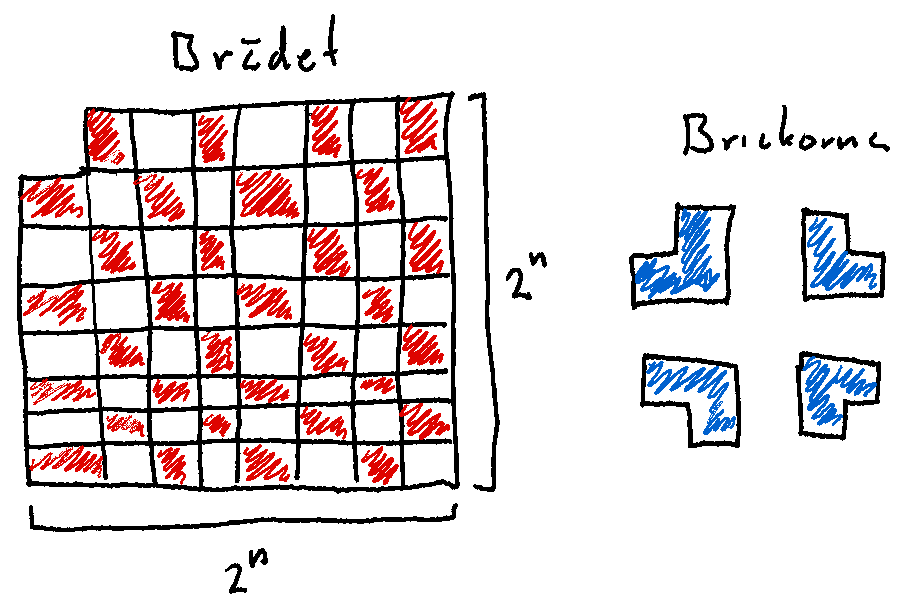
\includegraphics[width=0.9\textwidth]{graphics/chessboard_induction_extra_exercise.png}

  Ge ett induktionsbevis för att detta är möjligt för varje $n$.
\end{xca}

\begin{xca}
  För varje $n$ ges det $n$te \emph{Bell-talet} av
  $$B_n = \sum_{k=1}^{n} \stirlingPart{n}{k}.$$

  \begin{itemize}
    \item Förklara varför $B_n$ räknar antalet mängdpartitioner av $[n]$, oavsett antal delar.
    \item Ge ett kombinatoriskt bevis för att
    $$B_{n+1} = \sum_{k=0}^{n} \binom{n}{k} B_k.$$
  \end{itemize}
\end{xca}

\begin{xca}
  De \emph{harmoniska talen} $H_n$ ges av
  $$H_n = 1 + \frac{1}{2} + \frac{1}{3} + \ldots + \frac{1}{n}$$
  för varje $n$. Vad är den ordinära genererande funktionen för $H_n$?\sidenote[][]{Ledtråd: Ett av de första exemplen vi gav på faltningar var hur vi kunde få fram den kumulativa summan av en följd $\{a_k\}_{k=0}^\infty$, det vill säga följden $a_0, a_0 + a_1, a_0 + a_1 + a_2, \ldots$, som en faltning mellan $a$ och en annan följd.
  
  Använd detta för att uttrycka genererande funktionen för $H_n$ som en faltning mellan $h_n = \left(1, \frac{1}{2}, \frac{1}{3}, \ldots\right)$ och en annan följd. För att hitta genererande funktionen av $h_n$, pröva att ta en integral.}
\end{xca}

\begin{xca}
  Ge ett kombinatoriskt bevis för att
  $$\sum_{k=0}^{n} k\binom{n}{k} = n 2^{n-1}.$$
\end{xca}

%\bibliography{references}
%\bibliographystyle{plainnat}

\end{document}
